% Sinh tự động từ docs/report/chapter3.md bởi build.py — sửa file Markdown, không sửa file này.
\section{Ứng dụng}\label{sec:ch3}

Chương này áp dụng cài đặt negFIN của nhóm \cite{negfin} cho hai bài toán thực tế theo yêu cầu đề: phân tích giỏ hàng trên dữ liệu bán lẻ và tìm pattern trên chuỗi DNA. Mọi frequent itemset đều do CLI \texttt{run.jl} của nhóm sinh ra (Baseline); Python chỉ dùng để chuyển dữ liệu gốc sang định dạng SPMF và hậu xử lý kết quả. Toàn bộ pipeline chạy lại được bằng notebook \nolinkurl{notebooks/demo.ipynb}.

\subsection{Quy trình chung}

Mỗi ứng dụng gồm bốn bước: (1) tải dữ liệu công khai và kiểm SHA-256 theo \nolinkurl{data/applications/manifest.toml}; (2) script \texttt{prepare.py} biến dữ liệu gốc thành file transaction SPMF (mỗi dòng một giao dịch, item là số nguyên dương) cùng bảng ánh xạ ID $\leftrightarrow$ ý nghĩa; (3) chạy negFIN với \texttt{minsup} là tỷ lệ thập phân, ngưỡng tuyệt đối \(m = \lceil \mathit{minsup}\cdot N\rceil\) với \(N\) là số transaction; (4) hậu xử lý: sinh luật kết hợp (ứng dụng A) hoặc so sánh pattern giữa các lớp (ứng dụng B), rồi giải mã ID thành tên để diễn giải.

Cả hai bộ dữ liệu lấy từ UCI Machine Learning Repository, giấy phép CC BY 4.0; dữ liệu gốc không đưa vào repo mà được notebook tải và kiểm checksum khi chạy.

\subsection{Ứng dụng 1 --- Phân tích giỏ hàng (Online Retail)}

\subsubsection{Mục tiêu}

Tìm các nhóm sản phẩm thường được mua cùng nhau và sinh luật kết hợp X $\Rightarrow$ Y để gợi ý bán kèm, đóng gói combo và bố trí trưng bày.

\subsubsection{Dữ liệu}

Online Retail \cite{retail} gồm 541.909 dòng hóa đơn của một cửa hàng trực tuyến tại Anh chuyên quà tặng, từ 01/12/2010 đến 09/12/2011 (DOI 10.24432/C5BW33). Mỗi dòng có \texttt{InvoiceNo}, \texttt{StockCode}, \texttt{Description}, \texttt{Quantity}, \texttt{InvoiceDate}, \texttt{UnitPrice}, \texttt{CustomerID}, \texttt{Country}. Theo mô tả của UCI, nhiều khách hàng của công ty là người bán sỉ.

\subsubsection{Tạo transaction}

Một hóa đơn là một transaction; item là \texttt{StockCode} sản phẩm (chuẩn hóa chữ hoa, trùng trong hóa đơn tính một lần). Bảng~\ref{tab:c3-I} liệt kê các bước lọc theo thứ tự.

\begin{table*}[!t]
\centering\footnotesize
\caption{Các bước lọc dữ liệu Online Retail}
\label{tab:c3-I}
\setlength{\tabcolsep}{4pt}
\begin{tabular}{llrr}
\hline
\textbf{Bước lọc} & \textbf{Lý do} & \textbf{Dòng} & \textbf{Hóa đơn} \\ \hline
Dữ liệu gốc &  & 541.909 & 25.900 \\
Bỏ hóa đơn không toàn số (\texttt{C…} hủy, \texttt{A…} điều chỉnh) & không phải giao dịch mua & 532.618 & 22.061 \\
Bỏ \texttt{Quantity} $\le$ 0 & trả hàng, ghi nhận hỏng & 531.282 & 20.725 \\
Bỏ \texttt{UnitPrice} $\le$ 0 & điều chỉnh kho & 530.103 & 19.959 \\
Chỉ giữ mã dạng \texttt{\textbackslash{}d\{5\}{[}A-Z{]}*} & bỏ phí vận chuyển, phí ngân hàng, voucher\ldots{} & 527.725 & 19.773 \\
\hline
\end{tabular}
\end{table*}

Kết quả có N = 19.773 transaction, 3.791 sản phẩm khác nhau, trung bình 26,2 sản phẩm mỗi hóa đơn. Các dòng thiếu \texttt{CustomerID} được giữ lại vì phân tích giỏ hàng chỉ cần nội dung hóa đơn. Sản phẩm được đánh ID theo thứ tự sắp xếp của mã, nên ánh xạ ổn định với cùng dữ liệu và quy tắc lọc; tên hiển thị là mô tả xuất hiện nhiều nhất của mỗi mã.

\subsubsection{Sinh luật kết hợp}

Với mỗi frequent itemset \(Z\) có ít nhất hai phần tử, sinh mọi luật \(X \Rightarrow Y\) với \(X \cup Y = Z\), \(X\) và \(Y\) khác rỗng và rời nhau. Gọi \(\sup(\cdot)\) là số transaction chứa tập đó và \(N\) là tổng số transaction; các độ đo là \cite{agrawal}, \cite{brin}:

\begin{equation}
\mathrm{supp}(X \Rightarrow Y) = \frac{\sup(X \cup Y)}{N},
\end{equation}

\begin{equation}
\mathrm{conf}(X \Rightarrow Y) = \frac{\sup(X \cup Y)}{\sup(X)},
\end{equation}

\begin{equation}
\mathrm{lift}(X \Rightarrow Y) = \frac{\mathrm{conf}(X \Rightarrow Y)}{\sup(Y)/N}.
\end{equation}

Lift lớn hơn 1 nghĩa là \(X\) và \(Y\) cùng xuất hiện nhiều hơn so với khi chúng độc lập.

Do mọi tập con của một frequent itemset cũng frequent, \(\sup(X)\) và \(\sup(Y)\) đều có sẵn trong output của negFIN, không cần quét lại dữ liệu. Phép tính được kiểm bằng ví dụ tính tay trên CSDL toy 5 giao dịch của nhóm: luật \(\{2\} \Rightarrow \{3\}\) có \(\sup(\{2,3\}) = 3\), \(\sup(\{2\}) = \sup(\{3\}) = 4\), nên confidence \(= 0{,}75\) và lift \(= 0{,}75/0{,}8 = 0{,}9375\); với minconf \(= 0\), 15 frequent itemset sinh đúng 50 luật (mỗi itemset \(k\) phần tử cho \(2^k - 2\) luật).

\subsubsection{Tham số và kết quả}

Bảng~\ref{tab:c3-II} cho thấy số mẫu tăng nhanh khi hạ minsup. Nhóm chọn \textbf{minsup = 0,01} (\(m = 198\) hóa đơn) để có itemset từ ba sản phẩm trở lên, và \textbf{minconf = 0,5}.

\begin{table}[!t]
\centering\footnotesize
\caption{negFIN trên Online Retail (N = 19.773)}
\label{tab:c3-II}
\setlength{\tabcolsep}{3pt}
\begin{tabular}{rrrr}
\hline
\textbf{minsup} & \textbf{min\_count} & \textbf{Số itemset} & \textbf{Dài nhất} \\ \hline
0,03 & 594 & 143 & 2 \\
0,02 & 396 & 395 & 3 \\
0,01 & 198 & 2.026 & 5 \\
\hline
\end{tabular}
\end{table}

Ở minsup 0,01 và minconf 0,5 có 962 luật, sinh từ 477 itemset; lift thấp nhất là 4,74, trung vị 12,03. Bảng~\ref{tab:c3-III} liệt kê mười luật có lift cao nhất. Tất cả thuộc họ sản phẩm HERB MARKER (que cắm đánh dấu chậu thảo mộc) và là các cách chia X/Y khác nhau của chỉ ba itemset: \{THYME, ROSEMARY, PARSLEY\} (luật 1--4), \{THYME, ROSEMARY, BASIL\} (5--8) và \{THYME, ROSEMARY\} (9--10); hai luật cùng một itemset có cùng support nhưng khác confidence vì mẫu số sup(X) khác nhau.

\begin{table}[!t]
\centering\footnotesize
\caption{Mười luật có lift cao nhất (minsup 0,01, minconf 0,5). Mọi sản phẩm là
HERB MARKER; chỉ ghi tên loại cây}
\label{tab:c3-III}
\setlength{\tabcolsep}{3pt}
\begin{tabular}{rlrrr}
\hline
\textbf{\#} & \textbf{X $\Rightarrow$ Y} & \textbf{Supp.} & \textbf{Conf.} & \textbf{Lift} \\ \hline
1 & THYME $\Rightarrow$ ROSEMARY + PARSLEY & 1,03\% (203) & 0,86 & 78,77 \\
2 & ROSEMARY + PARSLEY $\Rightarrow$ THYME & 1,03\% (203) & 0,94 & 78,77 \\
3 & THYME + PARSLEY $\Rightarrow$ ROSEMARY & 1,03\% (203) & 0,95 & 78,52 \\
4 & ROSEMARY $\Rightarrow$ THYME + PARSLEY & 1,03\% (203) & 0,85 & 78,52 \\
5 & THYME + BASIL $\Rightarrow$ ROSEMARY & 1,01\% (200) & 0,95 & 78,46 \\
6 & ROSEMARY $\Rightarrow$ THYME + BASIL & 1,01\% (200) & 0,83 & 78,46 \\
7 & ROSEMARY + BASIL $\Rightarrow$ THYME & 1,01\% (200) & 0,93 & 77,97 \\
8 & THYME $\Rightarrow$ ROSEMARY + BASIL & 1,01\% (200) & 0,84 & 77,97 \\
9 & THYME $\Rightarrow$ ROSEMARY & 1,12\% (221) & 0,93 & 76,83 \\
10 & ROSEMARY $\Rightarrow$ THYME & 1,12\% (221) & 0,92 & 76,83 \\
\hline
\end{tabular}
\end{table}

Vì Bảng~\ref{tab:c3-III} chỉ cho thấy một họ sản phẩm, Bảng~\ref{tab:c3-IV} dùng thêm một quy tắc khách quan để minh họa nhiều nhóm hơn: duyệt danh sách luật theo lift giảm dần, chỉ giữ luật không chứa sản phẩm nào đã xuất hiện ở các luật được giữ trước đó.

\begin{table*}[!t]
\centering\footnotesize
\caption{Mười luật lift cao nhất không trùng sản phẩm (minsup 0,01, minconf 0,5)}
\label{tab:c3-IV}
\setlength{\tabcolsep}{4pt}
\begin{tabular}{rlrrr}
\hline
\textbf{\#} & \textbf{X $\Rightarrow$ Y} & \textbf{Supp.} & \textbf{Conf.} & \textbf{Lift} \\ \hline
1 & HERB MARKER THYME $\Rightarrow$ HERB MARKER ROSEMARY + PARSLEY & 1,03\% & 0,86 & 78,77 \\
2 & HERB MARKER MINT $\Rightarrow$ HERB MARKER BASIL & 1,05\% & 0,87 & 70,81 \\
3 & REGENCY TEA PLATE PINK $\Rightarrow$ REGENCY TEA PLATE ROSES + GREEN & 1,29\% & 0,84 & 51,82 \\
4 & SET OF 3 WOODEN TREE DECORATIONS $\Rightarrow$ SET OF 3 WOODEN STOCKING
DECORATION & 1,11\% & 0,75 & 46,33 \\
5 & REGENCY SUGAR BOWL GREEN $\Rightarrow$ REGENCY MILK JUG PINK & 1,23\% & 0,75 & 45,36 \\
6 & POPPY'S PLAYHOUSE LIVINGROOM $\Rightarrow$ POPPY'S PLAYHOUSE BEDROOM +
KITCHEN & 1,13\% & 0,68 & 43,14 \\
7 & JAM JAR WITH GREEN LID $\Rightarrow$ JAM JAR WITH PINK LID & 1,15\% & 0,74 & 42,94 \\
8 & PINK POLKADOT CUP $\Rightarrow$ BLUE POLKADOT CUP & 1,05\% & 0,68 & 41,22 \\
9 & CHILDRENS CUTLERY DOLLY GIRL $\Rightarrow$ CHILDRENS CUTLERY SPACEBOY & 1,15\% & 0,76 & 40,97 \\
10 & BLUE POLKADOT BOWL $\Rightarrow$ PINK POLKADOT BOWL & 1,05\% & 0,65 & 38,36 \\
\hline
\end{tabular}
\end{table*}

Hình~\ref{fig:c3-1} cho thấy phân bố của toàn bộ 962 luật: 93,7\% có support dưới 2\% và 79,1\% có lift dưới 20. Ba mươi hai luật có lift từ 60 trở lên đều thuộc họ HERB MARKER và có support không quá 1,12\%, nằm ở góc trái trên của hình; luật có support cao nhất (4,17\%, chứa JUMBO BAG PINK POLKADOT) chỉ có lift trung bình. Như vậy luật có lift cao nhất không phải luật phổ biến nhất.

\begin{figure}[!t]
\centering
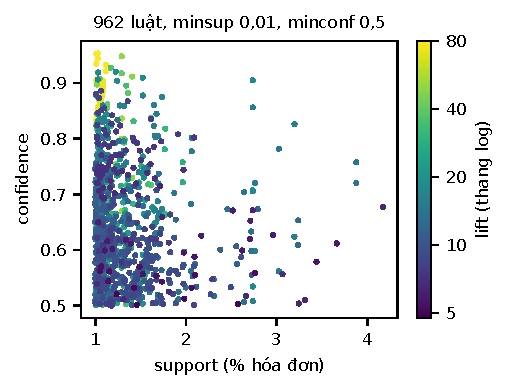
\includegraphics[width=\columnwidth]{retail-rules.pdf}
\caption{Support và confidence của 962 luật (minsup 0,01, minconf 0,5); màu biểu
diễn lift theo thang log.}
\label{fig:c3-1}
\end{figure}

\subsubsection{Diễn giải}

Các luật thể hiện hai kiểu hành vi mua:

\begin{itemize}
\tightlist
\item
  \textbf{Mua trọn bộ sưu tập} (herb marker, Poppy's Playhouse, đồ trang trí gỗ Giáng sinh): khách mua một mẫu thường mua tiếp các mẫu cùng dòng. Cửa hàng có thể bán theo bộ, hiển thị ``các mẫu còn lại trong bộ'' trên trang sản phẩm và trưng bày cạnh nhau.
\item
  \textbf{Phối nhiều màu của cùng một thiết kế} (bộ Regency, hũ mứt, cốc và bát polkadot, dao dĩa trẻ em bản girl/boy): khách lấy nhiều biến thể màu cùng lúc. Gợi ý là gói ``mix màu'' và nhập kho các màu theo tỷ lệ đi cùng nhau, tránh hết một màu làm mất cả đơn.
\end{itemize}

Confidence 0,65--0,95 nghĩa là phần lớn hóa đơn có vế trái cũng có vế phải; lift 38--79 cho biết các sản phẩm này xuất hiện cùng nhau nhiều gấp hàng chục lần so với khi được mua độc lập.

\subsubsection{Giới hạn}

Dữ liệu chỉ của một nhà bán lẻ trong một năm, và vì nhiều khách là người bán sỉ nên luật phản ánh hành vi nhập hàng theo bộ nhiều hơn người tiêu dùng lẻ. Lift nhạy với sản phẩm hiếm: support riêng của các sản phẩm trong Bảng~\ref{tab:c3-III} và \ref{tab:c3-IV} chỉ khoảng 1,2--1,9\%, nên cần đọc lift cùng support và confidence. minsup 0,01 bỏ qua sản phẩm có ít hơn 198 hóa đơn, do đó không thấy luật của mặt hàng ngách. Cuối cùng, luật chỉ thể hiện đồng xuất hiện, không phải quan hệ nhân quả.

\subsection{Ứng dụng 2 --- Pattern trên chuỗi DNA (Splice-junction)}

\subsubsection{Mục tiêu}

Kiểm tra xem negFIN có tự tìm ra các tín hiệu trình tự đặc trưng ở vị trí cắt nối (splice junction) hay không, bằng cách khai thác pattern riêng từng lớp chuỗi rồi so sánh giữa các lớp.

\subsubsection{Dữ liệu}

Bộ Splice-junction Gene Sequences \cite{splice} (DOI 10.24432/C5M888) gồm 3.190 chuỗi DNA linh trưởng lấy từ GenBank 64.1, mỗi chuỗi 60 base, ứng với vị trí −30 đến −1 và +1 đến +30; điểm nối nằm giữa −1 và +1. Có ba lớp: EI --- ranh giới exon$\rightarrow$intron (donor), 767 chuỗi; IE --- ranh giới intron$\rightarrow$exon (acceptor), 768 chuỗi; N --- không phải điểm nối, 1.655 chuỗi. File mô tả của nguồn ghi ngược donor/acceptor ở một mục; chương này dùng cách gọi khớp với phần mô tả bài toán của nguồn và với sinh học: EI là donor, IE là acceptor.

\subsubsection{Tạo transaction}

Mỗi chuỗi \(s\) là một transaction \(T(s)\); item là cặp vị trí--base, ký hiệu \texttt{p\textless{}vị\ trí\textgreater{}\_\textless{}base\textgreater{}}. Ví dụ, chuỗi EI đầu tiên của tập dữ liệu (ATRINS-DONOR-521) bắt đầu bằng \texttt{CCA…}, có \texttt{G} ở −1, \texttt{GT} ở +1..+2 và kết thúc bằng \texttt{G}, nên \(T(s)\) = \{\texttt{p-30\_C}, \texttt{p-29\_C}, \texttt{p-28\_A}, \ldots, \texttt{p-1\_G}, \texttt{p+1\_G}, \texttt{p+2\_T}, \ldots, \texttt{p+30\_G}\}, gồm 60 item. Với 60 vị trí và 4 base có 240 item; ID cố định \(\mathit{id} = 4j + b + 1\), với \(j \in \{0,\ldots,59\}\) là chỉ số vị trí và \(b \in \{0,1,2,3\}\) là chỉ số base theo thứ tự A, C, G, T, nên ánh xạ không phụ thuộc dữ liệu. Base mơ hồ (N, D, S, R; xuất hiện ở 15 chuỗi) không sinh item tại vị trí đó, nên các chuỗi này có ít hơn 60 item. Mã hóa kèm vị trí khiến mỗi transaction có tối đa một item cho mỗi vị trí, giữ được thông tin ``base nào ở vị trí nào'' dù itemset là tập hợp không có thứ tự. Các chuỗi trùng của nguồn (185 chuỗi) được giữ nguyên và được đếm như các transaction riêng.

Gọi \(D_c\) là tập chuỗi của lớp \(c \in \{\mathrm{EI}, \mathrm{IE}, \mathrm{N}\}\). negFIN chạy riêng trên từng \(D_c\) với ngưỡng \(m_c = \lceil \mathit{minsup}\cdot|D_c|\rceil\), và support theo lớp của itemset \(I\) được tính trên đúng mẫu số của lớp đó:

\begin{equation}
\mathrm{supp}_c(I) = \frac{|\{s \in D_c : I \subseteq T(s)\}|}{|D_c|}.
\end{equation}

Để so sánh, với mỗi itemset \(I\) của lớp đích \(c\), nhóm đếm lại \(\mathrm{supp}_{c'}(I)\) ở cả ba lớp trực tiếp từ transaction và tính độ tăng (growth) \cite{dongli} so với các lớp còn lại gộp chung \(D_{\neg c} = \bigcup_{c' \neq c} D_{c'}\):

\begin{equation}
\mathrm{growth}_c(I) = \frac{\mathrm{supp}_c(I)}{\mathrm{supp}_{\neg c}(I)},
\end{equation}

trong đó \(\mathrm{supp}_{\neg c}(I)\) tính theo công thức trên với mẫu số \(|D_{\neg c}|\); growth \(= \infty\) khi \(I\) không xuất hiện ở lớp nào khác. Vì lớp N có số chuỗi gấp khoảng hai lần EI hoặc IE, \(\mathrm{supp}_{\neg c}\) là tỷ lệ có trọng số theo kích thước lớp, không phải trung bình cộng của hai tỷ lệ.

\subsubsection{Tham số và kết quả}

\begin{table}[!t]
\centering\footnotesize
\caption{Số itemset theo lớp và minsup}
\label{tab:c3-V}
\setlength{\tabcolsep}{3pt}
\begin{tabular}{lrrrr}
\hline
\textbf{Lớp} & \textbf{N chuỗi} & \textbf{minsup 0,5} & \textbf{0,3} & \textbf{0,2} \\ \hline
EI & 767 & 35 & 280 & 2.375 \\
IE & 768 & 7 & 331 & 1.284 \\
N & 1.655 & 0 & 0 & 240 \\
\hline
\end{tabular}
\end{table}

Bảng~\ref{tab:c3-V} cho số itemset của từng lớp ở ba mức minsup. Nhóm chọn \textbf{minsup = 0,3} cho phân tích chính. Lớp N không có itemset nào ở 0,3; ở 0,2 có đủ 240 item đơn (mỗi base ở mỗi vị trí chiếm khoảng 25\%) nhưng không có cặp nào. Lớp N vì vậy đóng vai trò đối chứng: chuỗi không phải điểm nối không có tín hiệu gắn với vị trí.

Ở minsup 0,5, các item có mặt ở ít nhất một nửa số chuỗi là: với EI, \texttt{p-2\_A} (58\%), \texttt{p-1\_G} (81\%), \texttt{p+1\_G} (99,7\%), \texttt{p+2\_T} (99,0\%), \texttt{p+4\_A} (72\%), \texttt{p+5\_G} (86\%); với IE, \texttt{p-3\_C} (79\%), \texttt{p-2\_A} (99,6\%), \texttt{p-1\_G} (99,7\%).

Hình~\ref{fig:c3-2} tóm tắt tần suất của từng base ở từng vị trí trong mỗi lớp. Mỗi ô là support của một itemset một phần tử \texttt{p\textless{}vị\ trí\textgreater{}\_\textless{}base\textgreater{}} trong lớp đó, đếm trực tiếp từ transaction để có đủ 240 item; hình chỉ mang tính mô tả và giúp đọc các itemset nhiều phần tử ở Bảng~\ref{tab:c3-VI}. Ở EI, các ô đậm tập trung ở −1 (G), +1 (G), +2 (T) và +5 (G); ở IE, ở −3 (C), −2 (A), −1 (G), cùng một dải C/T nhạt hơn trải từ khoảng −20 đến −5; lớp N gần như đồng đều.

\begin{figure*}[!t]
\centering
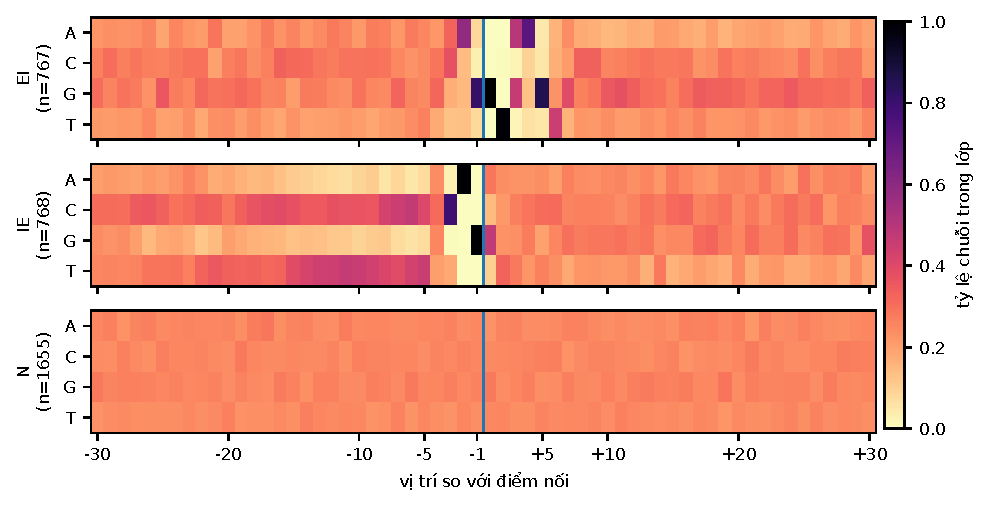
\includegraphics[width=\textwidth]{splice-positions.pdf}
\caption{Tỷ lệ chuỗi có mỗi base tại mỗi vị trí, theo lớp. Đường dọc đánh dấu
điểm nối giữa −1 và +1.}
\label{fig:c3-2}
\end{figure*}

Bảng~\ref{tab:c3-VI} liệt kê các itemset có growth cao nhất của EI và IE.

\begin{table*}[!t]
\centering\footnotesize
\caption{Itemset có growth cao nhất của mỗi lớp (minsup 0,3); support tính theo
từng lớp}
\label{tab:c3-VI}
\setlength{\tabcolsep}{4pt}
\begin{tabular}{llrrrr}
\hline
\textbf{Lớp} & \textbf{Itemset} & \textbf{EI} & \textbf{IE} & \textbf{N} & \textbf{Growth} \\ \hline
EI & p+1\_G p+2\_T p+4\_A p+5\_G p+6\_T & 30,2\% & 0,0\% & 0,0\% & $\infty$ \\
EI & p+1\_G p+2\_T p+5\_G p+6\_T & 40,3\% & 0,1\% & 0,1\% & 488 \\
EI & p+1\_G p+2\_T p+4\_A p+5\_G & 63,8\% & 0,9\% & 0,1\% & 193 \\
EI & p-1\_G p+1\_G p+2\_T p+4\_A p+5\_G & 47,3\% & 0,9\% & 0,0\% & 164 \\
IE & p-12\_T p-3\_C p-2\_A p-1\_G & 3,4\% & 33,2\% & 0,4\% & 25,1 \\
IE & p-10\_T p-3\_C p-2\_A p-1\_G & 2,9\% & 32,9\% & 0,6\% & 24,9 \\
IE & p-11\_T p-3\_C p-2\_A p-1\_G & 3,8\% & 37,1\% & 0,7\% & 22,5 \\
IE & p-7\_C p-3\_C p-2\_A p-1\_G & 5,1\% & 35,9\% & 0,3\% & 19,8 \\
\hline
\end{tabular}
\end{table*}

\subsubsection{Diễn giải}

Kết quả được đối chiếu với trình tự consensus đã công bố cho intron loại GT-AG: donor \texttt{MAG\textbar{}GTRAGT} và acceptor \texttt{(Y)n\ N\ CAG\textbar{}G} \cite{shapiro}.

\begin{itemize}
\tightlist
\item
  \textbf{Donor (EI).} negFIN tìm lại gần như đủ consensus donor: \texttt{G} ở −1 (kèm \texttt{A} ở −2) phía exon, \texttt{GT} ở +1..+2, rồi \nolinkurl{A/G} ở +3, \texttt{A} ở +4, \texttt{G} ở +5, \texttt{T} ở +6. Riêng cặp \texttt{GT} ở +1..+2 có mặt ở 99,0\% chuỗi EI, so với 14,1\% ở IE và 5,9\% ở N. Itemset năm phần tử \texttt{p+1\_G\ p+2\_T\ p+4\_A\ p+5\_G\ p+6\_T} xuất hiện ở 30,2\% chuỗi EI và không có ở lớp nào khác.
\item
  \textbf{Acceptor (IE).} Bộ ba \texttt{CAG} ở −3..−1 có mặt ở 78,8\% chuỗi IE, so với 22,8\% ở EI và 2,3\% ở N; riêng \texttt{AG} ở −2..−1 đạt 99,5\%. Các itemset đặc trưng nhất của IE ghép \texttt{CAG} với một base \texttt{T} hoặc \texttt{C} ở vị trí −6..−17, tức vùng giàu pyrimidine (polypyrimidine tract) nằm trước acceptor. Kiểm tra trực tiếp: tỷ lệ pyrimidine ở vùng −20..−5 là 77,4\% với IE, so với 49,1\% với EI và 49,3\% với N.
\item
  Growth của IE thấp hơn EI vì tín hiệu acceptor phân tán: vùng pyrimidine không cố định vị trí nên mỗi vị trí chỉ đạt khoảng 30--40\%, trong khi tín hiệu donor tập trung ở vài vị trí gần như cố định.
\end{itemize}

\subsubsection{Giới hạn}

Itemset chỉ biểu diễn đồng xuất hiện của các base ở vị trí tuyệt đối, không có thứ tự hay khoảng cách tương đối; vì vậy một motif có thể dịch vị trí như polypyrimidine tract bị tách thành nhiều itemset rời rạc. Growth chỉ mô tả mức đặc trưng trên chính dữ liệu này: không có tập kiểm tra riêng, không có kiểm định thống kê, nên không phải bằng chứng về khả năng phân lớp chuỗi mới; growth = $\infty$ của itemset EI trong Bảng~\ref{tab:c3-VI} cũng chỉ có nghĩa là không quan sát thấy ở 2.423 chuỗi IE và N (768 + 1.655). Các chuỗi trùng được đếm nhiều lần nên support có thể lệch nhẹ so với tập chuỗi duy nhất. Dữ liệu từ năm 1991, chỉ gồm gen linh trưởng và điểm nối GT-AG, nên không suy rộng cho loài khác hay các loại intron hiếm. Chương này chỉ khẳng định các pattern khớp với consensus đã công bố; các pattern còn lại được xem là quan sát.

\subsection{Tái lập và kiểm chứng}

Notebook \nolinkurl{notebooks/demo.ipynb} dùng Julia có sẵn hoặc tự cài Julia 1.12.0 (kiểm SHA-256), lấy mã nguồn ở commit chỉ định, tải hai bộ dữ liệu và kiểm checksum, rồi chạy lần lượt ví dụ toy, ứng dụng 1 và ứng dụng 2 qua \texttt{run.jl}; cell cuối in commit, phiên bản Julia và mọi tham số. Notebook đã được chạy Run all trên runtime Colab mới ở commit \texttt{7e3e9b0} với Julia 1.12.6, cho đúng các số liệu trong chương này; bản có output được chia sẻ công khai tại liên kết trong README. Các bước kiểm chứng đã thực hiện:

\begin{itemize}
\tightlist
\item
  12 unit test Python cho tiền xử lý, sinh luật và so sánh lớp, gồm ví dụ tính tay trên CSDL toy.
\item
  19 luật khác nhau trong Bảng~\ref{tab:c3-III} và \ref{tab:c3-IV} được tính lại support, confidence, lift trực tiếp từ file transaction, không qua negFIN: khớp hoàn toàn.
\item
  Script so sánh lớp đếm lại support của toàn bộ 611 itemset (EI 280, IE 331) từ transaction và báo lỗi nếu khác output của negFIN: không có sai lệch.
\end{itemize}
